\documentclass[%
reprint,
superscriptaddress,
%groupedaddress,
%unsortedaddress,
%runinaddress,
%frontmatterverbose,
%preprint,
showpacs,preprintnumbers,
%nofootinbib,
%nobibnotes,
%bibnotes,
 amsmath,amssymb,
 aps,
%pra,
%prb,
prd,
%prl,
%rmp,
%prstab,
%prstper,
%floatfix,
]{revtex4-1}

\usepackage{float}
\usepackage{graphicx}% Include figure files
\usepackage{dcolumn}% Align table columns on decimal point
\usepackage{bm}% bold math
\usepackage{bbold}
\usepackage{amssymb,amsmath}
\usepackage{hyperref}% add hypertext capabilities
%\usepackage[mathlines]{lineno}% Enable numbering of text and display math
%\linenumbers\relax % Commence numbering lines

%\usepackage[showframe,%Uncomment any one of the following lines to test
%%scale=0.7, marginratio={1:1, 2:3}, ignoreall,% default settings
%%text={7in,10in},centering,
%%margin=1.5in,
%%total={6.5in,8.75in}, top=1.2in, left=0.9in, includefoot,
%%height=10in,a5paper,hmargin={3cm,0.8in},
%]{geometry}



\usepackage{color}
\usepackage{amsfonts}
\usepackage{subfigure}
\usepackage{array}


\newcommand{\Tr}{\ensuremath{\operatorname{Tr}}}
\newcommand{\tr}{\ensuremath{\operatorname{tr}}}
\newcommand{\Omegaqq}{\ensuremath{\Omega_{\bar{q}q}}}
\newcommand{\vev}[1]{\ensuremath{\left\langle #1 \right\rangle}}
\newcommand{\einh}[1]{\ensuremath{\,\text{#1}}}
\newcolumntype{L}{>{\centering\arraybackslash}m{3cm}}



\newcommand{\overbar}[1]{\mkern 1.5mu\overline{\mkern-1.5mu#1\mkern-1.5mu}\mkern 1.5mu}

\definecolor{bjcol}{rgb}{1,.44,0.13}

% color def's

\definecolor{blue}{rgb}{0,0,1}
\newcommand{\colb}[1]{{\color{blue} #1}}
\definecolor{green}{rgb}{0,1,0}
\newcommand{\colg}[1]{{\color{green} #1}}
\definecolor{red}{rgb}{1,0,0}
\newcommand{\colr}[1]{{\color{red} #1}}
\newcommand{\colJ}[1]{{\color{cyan} #1}}
\definecolor{gray}{rgb}{.5,.5,.5}
\newcommand{\drop}[1]{{\sout{ {\color{gray} #1}}}}
\definecolor{darkgreen}{rgb}{.0,.5,.0}
\newcommand{\colL}[1]{{\color{darkgreen} #1}}


\def\Fig#1{Fig.~\ref{#1}} \def\Tab#1{Tab.~\ref{#1}}
\def\Figs#1{Figs.~\ref{#1}} \def\Tab#1{Tab.~\ref{#1}}
\def\Eqs#1{Eqs.~(\ref{#1})}
\def\Eq#1{Eq.~(\ref{#1})}
\def\eq#1{(\ref{#1})}
\def\eqref#1{(\ref{#1})}
\def\fig#1{Fig.~\ref{#1}}
\def\tab#1{Tab.~\ref{#1}}
\def\eqs#1{(\ref{#1})}
\def\Eqs#1{(\ref{#1})}
\def\sec#1{Sec.~\ref{#1}}
\def\app#1{Appendix~\ref{#1}}
\newcommand{\Phibar}{\ensuremath{\bar{\Phi}}}
\newcommand{\LPQM}{\ensuremath{\mathcal{L}_{\textrm{PQM}}}\xspace}

\def\dbar{{\mathchar'26\mkern-12mu d}}
\def\lA0{{\langle A_0 \rangle}}
\def\bA0{{\bar{A}_0}}
\def\lLA{{\langle L[A_0] \rangle}}
\def\lL{{\langle L \rangle}}
\def\lLc{{\langle L^\dagger \rangle}}
\def\lLAc{{\langle L^\dagger[A_0] \rangle}}


\def\dr{{D\!\llap{/}}\,}
\def\Dr{{D\!\llap{/}}\,}
\def\ipv{\vec{p}\llap{/}}
\def\pslash{p\llap{/}}

\def\0#1#2{\frac{#1}{#2}}

\newcommand{\bsig}{\ensuremath{\bar{\sigma}}}
\newcommand{\lsm}{L\ensuremath{\sigma}M\xspace}
\newcommand{\pT}{\ensuremath{T_0}}
\newcommand{\Tl}{\ensuremath{T_\chi}}
\newcommand{\Ts}{\ensuremath{T_\chi^s}}
\newcommand{\Tchi}{\ensuremath{T_\chi}}
\newcommand{\Td}{\ensuremath{T_d}}
\newcommand{\Tc}{\ensuremath{T_c}}
\newcommand{\muc}{\ensuremath{\mu_c}}
\newcommand{\coloronl}{(color online)\xspace}

\newcommand{\mrm}[1]{\mathrm{#1}}
\def\qbar{\bar{q}}
\newcommand{\sx}{\sigma_{x}}
\newcommand{\sy}{\sigma_{y}}

\newcommand{\tkcomment}[1]{\textcolor{blue}{#1}}
\newcommand{\tkremark}[1]{\textcolor{blue}{[#1]}}
\newcommand{\jlcomment}[1]{\textcolor{green}{[#1]}}
\newcommand{\wjfu}[1]{\textcolor{red}{[#1]}}

%
%%%%%%%%%%%%%%%%%%%%%%%%%%%%%%%%%%%%%%%%%%%%%%%%%%%%%%%%%%%%%%%%%%%%%%%%%%%%%

\graphicspath{{./figures/}{./}}

\begin{document}

\preprint{}

\title{Nontrivial dispersion relation and QCD thermodynamics in the low energy effective model
}

\author{Shi Yin}
% \email{}
\affiliation{School of Physics, Dalian University of Technology, Dalian, 116024,
  P.R. China}

\author{Rui Wen}
\affiliation{School of Physics, Dalian University of Technology, Dalian, 116024,
  P.R. China}

\author{Wei-jie Fu}
\email{wjfu@dlut.edu.cn}
\affiliation{School of Physics, Dalian University of Technology, Dalian, 116024,
  P.R. China}

%\date{\today}% It is always \today, today,
             %  but any date may be explicitly specified

\begin{abstract}
We study the...
\end{abstract}

%\pacs{Valid PACS appear here}% PACS, the Physics and Astronomy
\pacs{11.30.Rd, %Chiral symmetries
         11.10.Wx, %Finite-temperature field theory
         05.10.Cc, %Renormalization group methods
         12.38.Mh  %Quark-gluon plasma
     }                             % Classification Scheme.
%\keywords{Suggested keywords}%Use showkeys class option if keyword
                              %display desired
\maketitle

%\tableofcontents

%%%%%%%%%%%%%%%%%%%%%%%%%%%%%%%%%%%%%%%%%%%%%%%%%%%%%%%%%%%
%%%%%%%%%%%%%%%%%%%%%%%%%%%%%%%%%%%%%%%%%%%%%%%%%%%%%%%%%%%
\section{Introduction}


The past years have  ....


%%%%%%%%%%%%%%%%%%%%%%%%%%%%%%%%%%%%
\section{low-energy effective models under the FRG}
As is shown in the previous work(see[??]), the low-energy effective theory can be studied with the flow equation of the 
scale-dependent effective action $
\Gamma_k[\Phi]$, $\Phi$ is the superfield, it can be written as
 $\Phi=(A_\mu,c,\overline{c},q,\overline{q},\phi,...)$.  The flow equation within the framework of FRG can be written as
\begin{align}
\partial_t\Gamma_k[\Phi]=\frac{1}{2}TrG_{\Phi\Phi}[\Phi]\partial_tR_k^\Phi,\qquad t=ln(k/\Lambda)
\label{eq:floweq}
\end{align}
where
\begin{align}
G_{\Phi_i\Phi_j}[\Phi]=\left(\frac{1}{\frac{\delta^2\Gamma_k[\Phi]}{\delta\Phi^2}+R^\Phi_k}\right)_{ij}
\end{align}
is the propagator which is full field-dependent.
The effective action that depends on the scale of the quark-meson model can be written like this
\begin{align}
\begin{split}
\Gamma_k=\int_x\{Z_{q,k}\overline{q} (\gamma_\mu \partial_\mu -\gamma_0(\mu+igA_0) )q+\frac{1}{2}Z_{\phi,k}
(\partial_\mu \phi)^2\\+h_k\overline{q}
(T^0\sigma+i\gamma_5\vec{T}\cdot\vec{\pi})q+V_k(\rho)-c\sigma \}+\cdot\cdot\cdot\label{eq:effact}
\end{split}
\end{align}
here we omited the higher-order terms. The integral sign can be written as $\int_x=\int_x^{1/T}dx_0\int d^3x$.The meson 
field is $\phi=\left(\sigma,\vec{\pi}
\right)$ . 
$V_k(\rho)$ is field-dependent effective potential which is $O(4)$ invariant, with $\rho=\phi^2/2$.The $k$ is the infrared 
cutoff scale in FRG, see [??]; $
\Lambda$ 
is some reference scale ; $\mu$ is the chemical potential of quark. ($T^0$,$\bm{T}$) is the generators of flavor space with  
$\mathrm{tr}(T^{i}T^{j})=\frac{1}
{2}\delta^{ij}$ and
 $T^{0}=\frac{1}{\sqrt{2N_{f}}}\mathbb{1}_{N_{f}\times N_{f}}$. The linear term $-c\sigma$ breaks the chiral symmetry. At 
 the same time, the linear breaking 
 parameter $c$ is proportional to the mass of $\vec{\pi}$; $h_k$ is the Yukawa coupling. The flow equation in \Eq{eq:floweq} is shown in \Fig{fig:fe}. More details see \cite{?}.\\
%%%%%%%%%%%%%%%%%%%%%%%%%%%%%%%%%%%%
\begin{figure}[h]
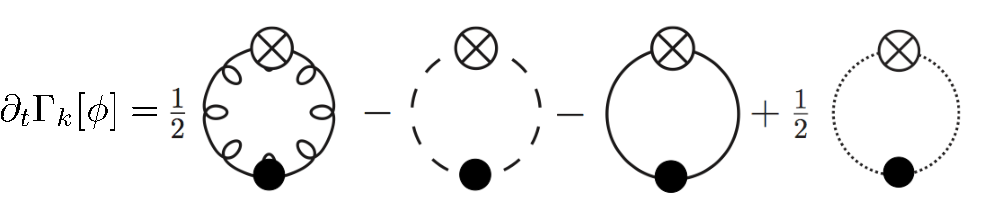
\includegraphics[width=0.45\textwidth]{FRG-QCD_rebosonised.pdf}
\caption{The first two diagrams stand for the glue contribution; the other two stand for the quark and mesonic contribution }
\label{fig:fe}
\end{figure}
%%%%%%%%%%%%%%%%%%%%%%%%%%%%%%%%%%%%
Then, we can divide the effective action like
\begin{align}
\begin{split}
&\Gamma_{k}[\Phi]=\Gamma_{glue,k}[\Phi]+\Gamma_{matt,k}[\Phi],\\
&\Gamma_{matt,k}=\Gamma_{q,k}+
\Gamma_{\phi,k}
\label{}
\end{split}
\end{align}\\
%%%%%%%%%%%%%%%%%%%%%%%%%%%%%%%%%%%%
%%%%%%%%%%%%%%%%%%%%%%%%%%%%%%%%%%



\section{polyakov-quark-meson model under the FRG approximation}




%%%%%%%%%%%%%%%%%%%%%%%%%%%%%%%%%%%%%%%



\subsection{Flow equation}

\begin{align}\label{fqm}
\begin{split}
\partial_t\Gamma_k[\Phi]=\frac{1}{2}TrG_{\phi\phi}[\Phi]\partial_tR^{\phi}_{k}-TrG_{q\bar{q}}[\Phi]\partial_tR^{q}_{k}
\end{split}
\end{align}
\begin{align}\label{cqm}
\begin{split}
G_{\phi\phi/q\bar{q}}[\Phi]=\left( \frac{1}{\frac{\delta^2\Gamma_k[\Phi]}{\delta\Phi^2}+R^{\Phi}_{k}} \right)_{\phi\phi/
q\bar{q}}
\end{split}
\end{align}

\begin{align}\label{}
\begin{split}
\bar{\phi}=Z^{\frac{1}{2}}_{\phi,k}\phi ,\qquad \bar{h}_k=\frac{h_k}{Z_{q,k}Z^{\frac{1}{2}}_{\phi,k}}
\end{split}
\end{align}



%%%%%%%%%%%%%%%%%%%%%%%%%%%%%%%%%%%%%%%%%



\subsection{The flow equations of the effective potential}
The 3d regulators have been used in our calculation. The details see Appendix \ref{a}. Through the derivation of the 
effective action \ref{fqm} and \ref{cqm} we can get the flow equation of the effective potential under the constant mesonic
fields:
\begin{align}
\begin{split}
\partial_tV_k(\rho)=&\frac{k^4}{4\pi^2}[(N^2_f-1)l^{(B,4)}_{0}(\bar{m}^{2}_{\pi,k},\eta^{\bot}_{\phi,k};T)\\
&+l^{(B,4)}_{0}(\bar{m}^{2}_{\sigma,k},\eta^{\bot}_{\phi,k};T)\\
&-4N_cN_fl^{(F,4)}_{0}(\bar{m}^{2}_{q,k},\eta_{q,k};T,\mu)]
\end{split}
\end{align}
The $l_0^{(B/F,n)}$ is the threshold functions. The form of the threshold functions are given in the Appendix \ref{a}. Below 
are the quark mass and meson masses which are renormalized and dimensionless
\begin{align}
\begin{split}
\bar{m}^{2}_{\pi,k}&=\frac{V'_k(\rho)}{k^2Z^{\bot}_{\phi,k}}\\
\bar{m}^{2}_{\sigma,k}&=\frac{V'_k(\rho)+2\rho V''_k(\rho)}{k^2Z^{\bot}_{\phi,k}}\\
\bar{m}^{2}_{q,k}&=\frac{h^{2}_{k}\rho}{2k^2Z^{2}_{q,k}}
\end{split}
\end{align}
In the finite temperature the meson wave function renormalization $Z_{\phi,k}$ is split into $Z^\|$ and $Z^\bot$. In the past 
calculation we use a 
approximation that we assume $Z^\|=Z^\bot$. In this work, we abolished this approximation and observe if the change 
have any influence on the results.
By considering the difference between $Z^\bot_{\phi,k}$ and $Z^\|_{\phi,k}$ we can calculate the anomalous dimensions 
respectively.The defination of the 
anomalous dimensions is given by
\begin{align}
\eta_{\phi,k}^\bot=-\frac{\partial_tZ_{\phi,k}^\bot}{Z_{\phi,k}^\bot} ,\qquad \eta_{\phi,k}^\|=-\frac{\partial_tZ_{\phi,k}^\|}
{Z_{\phi,k}^\|}\label{eq:anodim}
\end{align}
and the definition of the quark anomalous dimension is
\begin{align}
\begin{split}
\eta_{q,k}=-\frac{\partial_tZ_{q,k}}{Z_{q,k}}
\end{split}
\end{align}
The frequency and spatial momentum are independent when we calculating the anomalous dimensions. And the 
frequency and spatial momenta are low when we deducing the anomalous dimensions. Some details of the meson 
anomalous dimensions are discussed in Appendix \ref{b} and quark anomalous dimension in Appendix \ref{c}.




Here we consider two expansion ways of the effective potential. On one hand, the Taylor expansion of the effective 
potential is about a field value $\kappa$ which is unrenormalised and fixed. The effective potential can be written as
\begin{align}\label{}
\begin{split}
\bar{V}_k(\bar{\rho})=\sum^{N}_{n=0}\frac{\bar{\lambda}_{n,k}}{n!}(\bar{\rho}-\bar{\kappa}_k)^n
\end{split}
\end{align}
with $\bar{\lambda}_{n,k}=\lambda_{n,k}/Z^{n}_{\phi,k}$ and $\bar{\kappa}_k=Z_{\phi,k}\kappa$.
The other hand, we make the expansion point $\kappa$ depends on the cutoff scales $k$. Then the $\bar{\kappa}_k$ 
can be written as
\begin{align}\label{}
\begin{split}
\bar{\kappa}_k=Z_{\phi,k}\kappa_k
\end{split}
\end{align} 

%%%%%%%%%%%%%%%%%%%%%%%%%%%%%%%%%%%%%%%


\subsection{Baryon number fluctuation and kurtosis}
The definition of the baryon number fluctuation is given by
\begin{align}\label{}
\begin{split}
\chi^{B}_{n}=\frac{\partial^n}{\partial(\mu_B/T)^n}\frac{p}{T^4}
\end{split}
\end{align} 
the baryon chemical potential $\mu_B=3\mu$. The quadratic and quartic fluctuations can be expressed using the 
average baryon number fluctuation $\langle N_B \rangle$
\begin{align}\label{}
\begin{split}
\chi^{B}_{2}&=\frac{1}{VT^3}\langle \delta {N_B}^2 \rangle\\
\chi^{B}_{4}&=\frac{1}{VT^3}\left( \langle \delta {N_B}^4 \rangle-3\langle \delta {N_B}^2 \rangle^2 \right)
\end{split}
\end{align}

The definition of the kurtosis can be written as
\begin{align}
\kappa \sigma^2=\frac{\chi^{B}_{4}}{\chi^{B}_{2}}
\end{align}


%%%%%%%%%%%%%%%%%%%%%%%%%%%%%%%%%%%




\subsection{numerical results}
In this section we will show the numerical compute results of the comparison. Two comparisons have been made, one is $Z^{\|}_{\phi}
=Z^{\bot}_{\phi}$ and $Z^{\|}_{\phi}\neq Z^{\bot}_{\phi}$, the other one is the fix point and physical point expansion of the effective 
potential. The meson mass is shown as a function of temperature, the difference between the red and blue line are very small. But 
the difference caused by the expansion method is large. The mesons' mass are much higher of the physical point expansion than the 
fix point. 

As is shown in the \Fig{fig:chi2chi4}, the baryon chemical potential has little influence to the numerical result of 
quadratic fluctuation. However, we can see clearly the influence of the change of wave function renormalization factors.


The results of the quartic fluctuations under two kinds of wave function renormalizations have larger difference at the peak
 of the curves, the results of $Z^{\bot}_{\phi,k}\neq Z^{\|}_{\phi,k} $ are lower than the results of $Z^{\bot}_{\phi,k}= Z^{\|}_{\phi,k} $.



\begin{figure*}[t]
\label{fig:mphi}
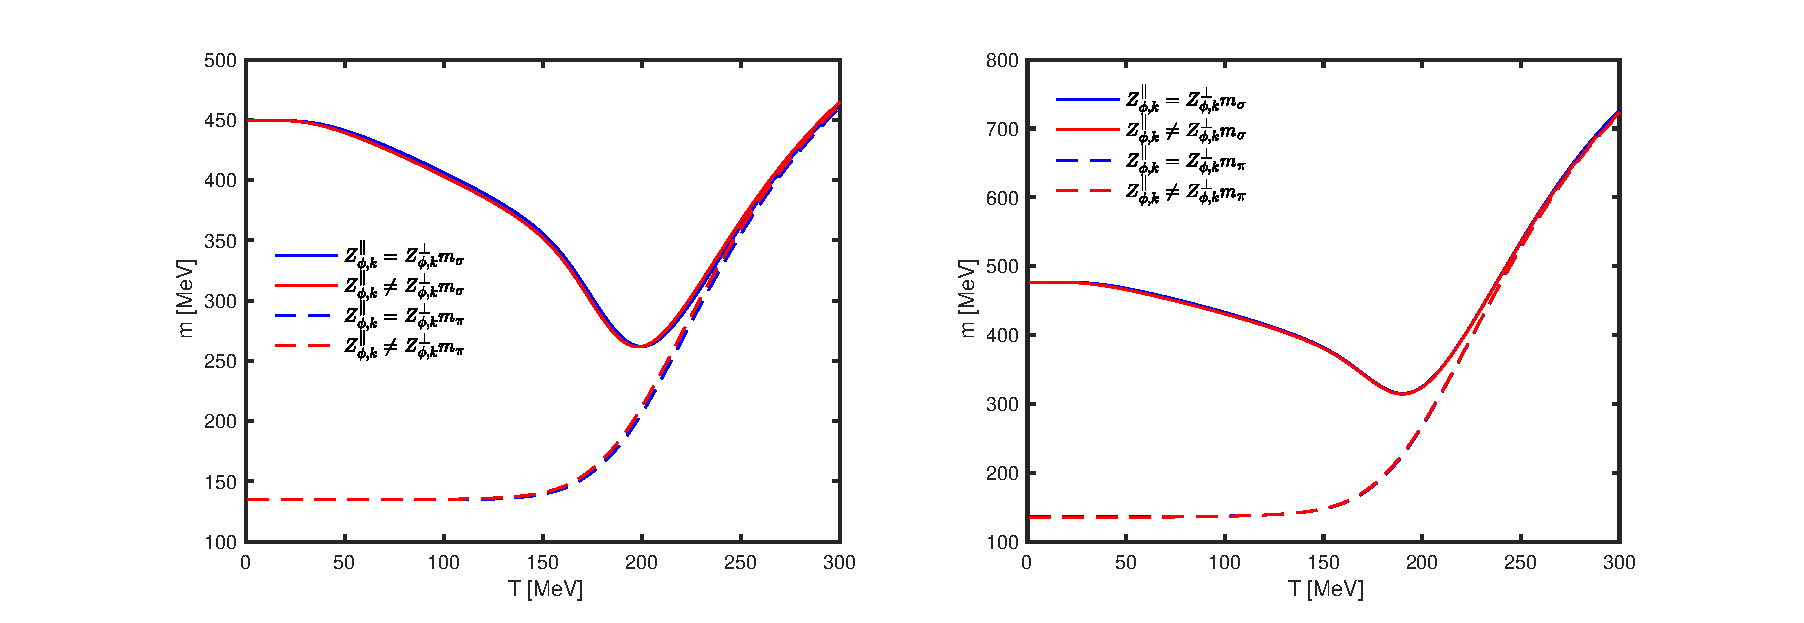
\includegraphics[width=1.0\textwidth]{mphi.eps}
\caption{blue color stands for the results with $Z^{\bot}_{\phi,k}=Z^{\|}_{\phi,k}$ and the red color stands for the $Z^{\bot}
_{\phi,k}\neq Z^{\|}_{\phi,k} $. The left diagram is the results under the fix-point-expansion of the effective potential, and 
the right picture is the results of the physical-point-expansion.}
\end{figure*}








\begin{figure}[t]
\label{fig:trace}
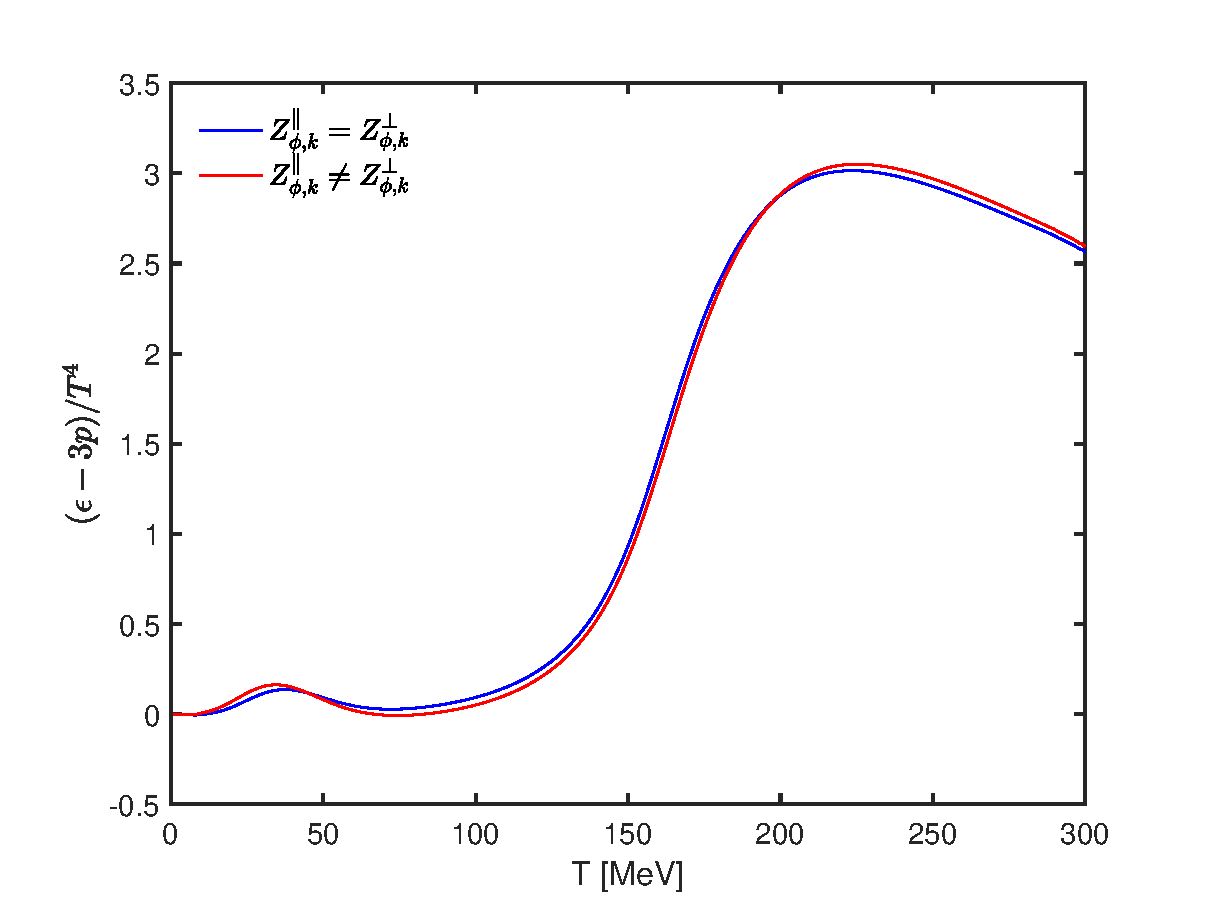
\includegraphics[width=0.46\textwidth]{trace.eps}
\caption{}
\end{figure}





\begin{figure*}[t]
\label{fig:chi2chi4}
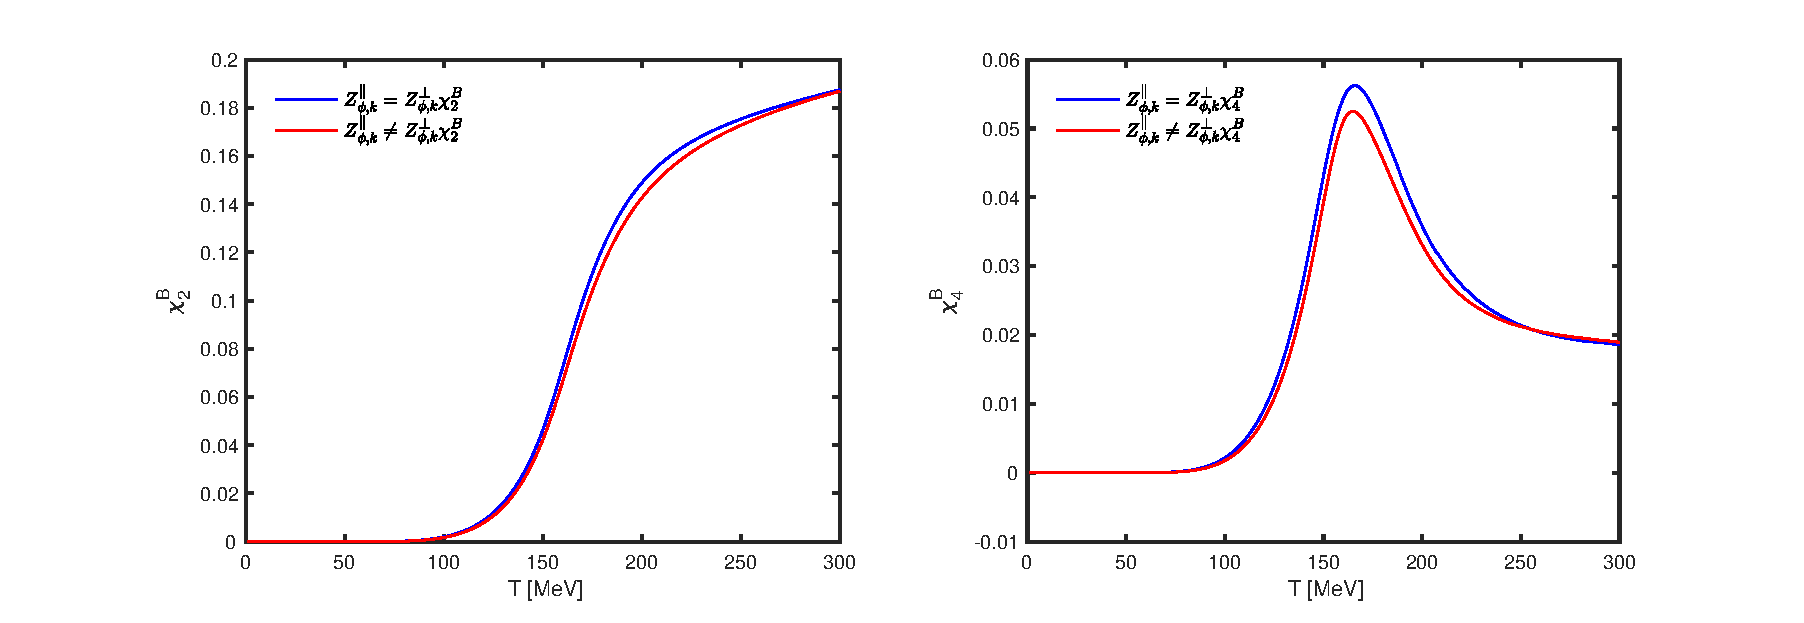
\includegraphics[width=1.0\textwidth]{chi2chi4.eps}
\caption{blue color stands for the results with $Z^{\bot}_{\phi,k}=Z^{\|}_{\phi,k}$ and the red color stands for the $Z^{\bot}
_{\phi,k}\neq Z^{\|}_{\phi,k} $. The full and dotted lines are the results under the chemical potential of 50 MeV and 100 
MeV. These results are under the physical point expansion of the effective potential. }
\end{figure*}



\begin{figure*}[t]
\label{fig:chi13}
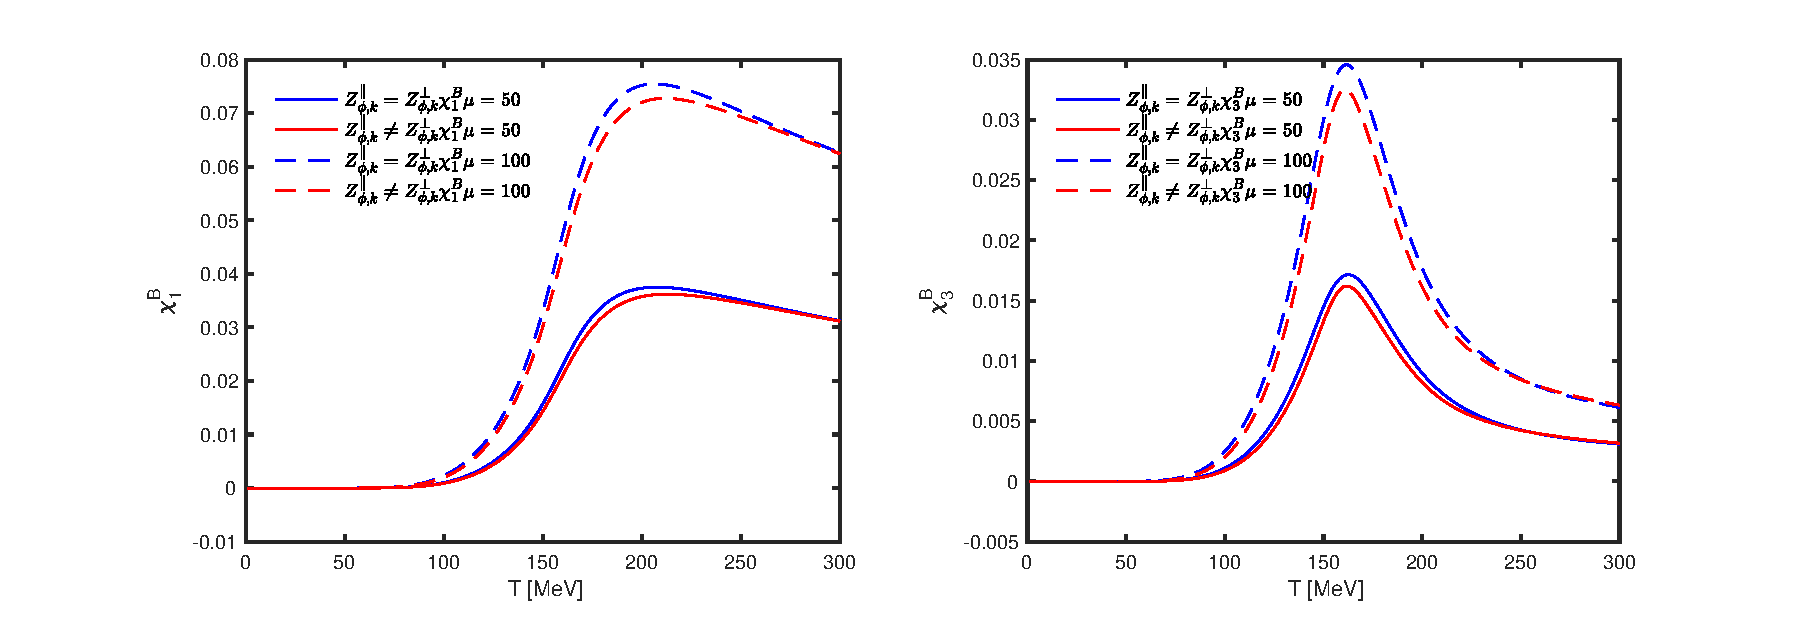
\includegraphics[width=1.0\textwidth]{chi13.eps}
\caption{blue color stands for the results with $Z^{\bot}_{\phi,k}=Z^{\|}_{\phi,k}$ and the red color stands for the $Z^{\bot}
_{\phi,k}\neq Z^{\|}_{\phi,k} $. The full and dotted lines are the results under the chemical potential of 50 MeV and 100 
MeV. These results are under the physical point expansion of the effective potential. }
\end{figure*}




\begin{figure}[t]
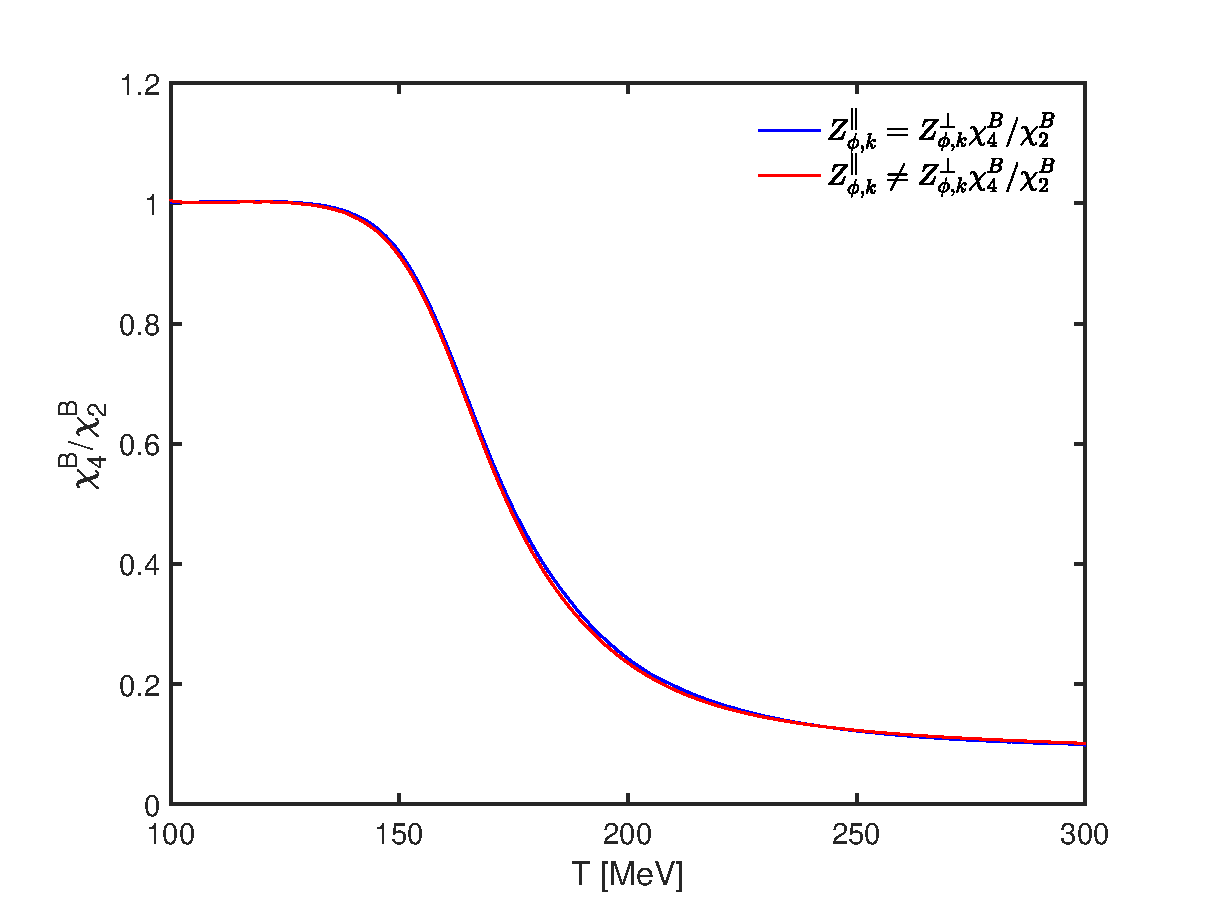
\includegraphics[width=0.46\textwidth]{r42.eps}
\caption{blue color stands for the results with $Z^{\bot}_{\phi,k}=Z^{\|}_{\phi,k}$ and the red color stands for the $Z^{\bot}
_{\phi,k}\neq Z^{\|}_{\phi,k} $.}
\label{fig:r42}
\end{figure}


\begin{figure}[t]
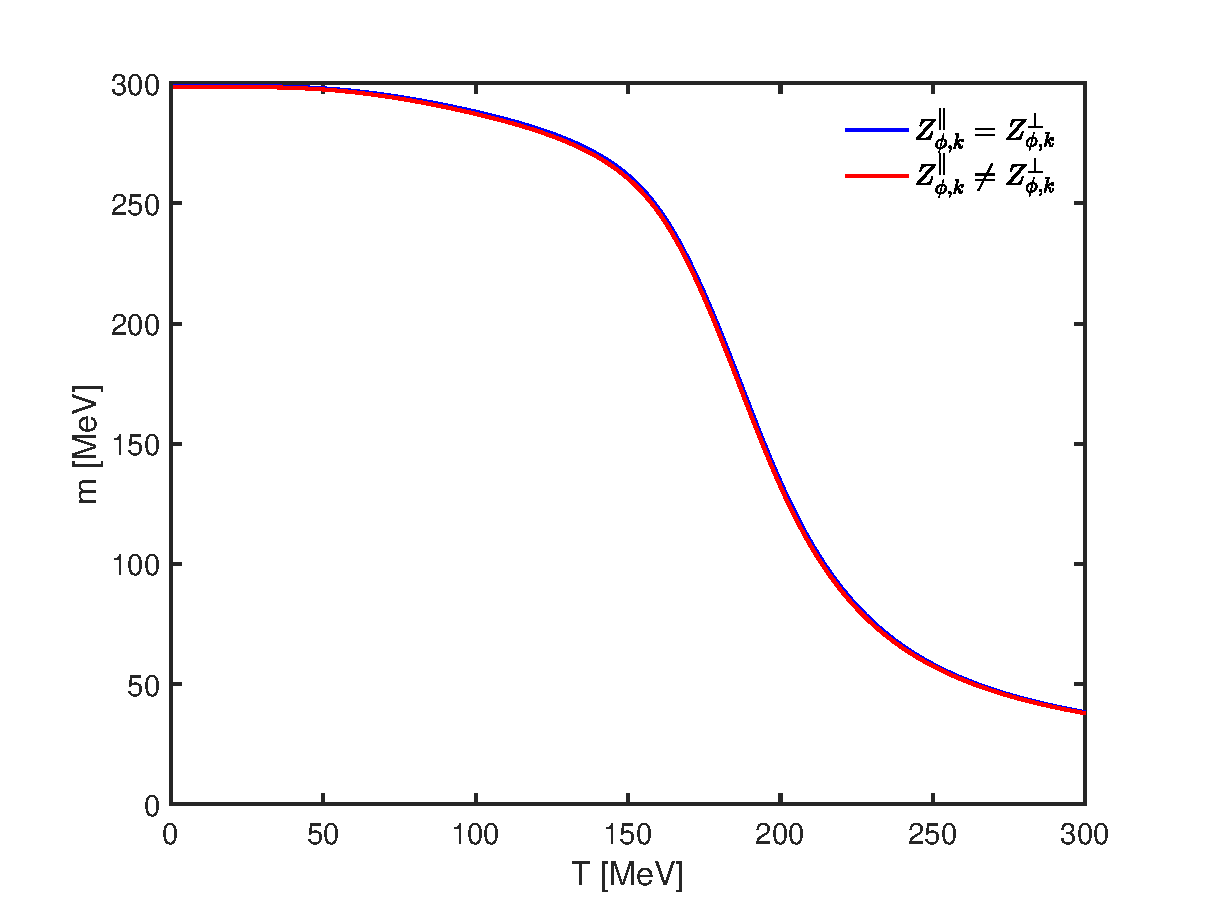
\includegraphics[width=0.46\textwidth]{mf.eps}
\caption{blue color stands for the results with $Z^{\bot}_{\phi,k}=Z^{\|}_{\phi,k}$ and the red color stands for the $Z^{\bot}
_{\phi,k}\neq Z^{\|}_{\phi,k} $.}
\label{fig:mf}
\end{figure}


\begin{figure}[t]
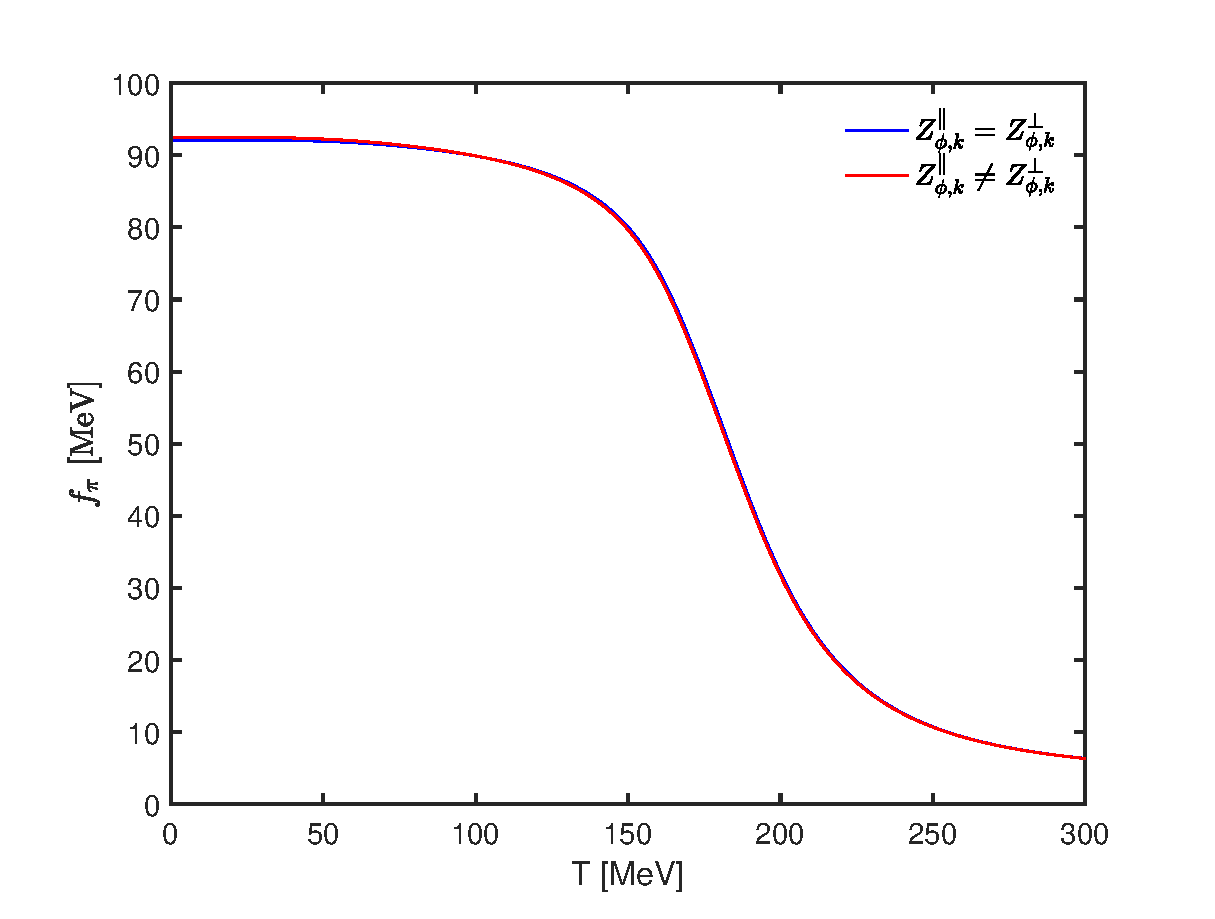
\includegraphics[width=0.46\textwidth]{fpi.eps}
\caption{blue color stands for the results with $Z^{\bot}_{\phi,k}=Z^{\|}_{\phi,k}$ and the red color stands for the $Z^{\bot}
_{\phi,k}\neq Z^{\|}_{\phi,k} $.}
\label{fig:fpi}
\end{figure}

\begin{figure}[t]
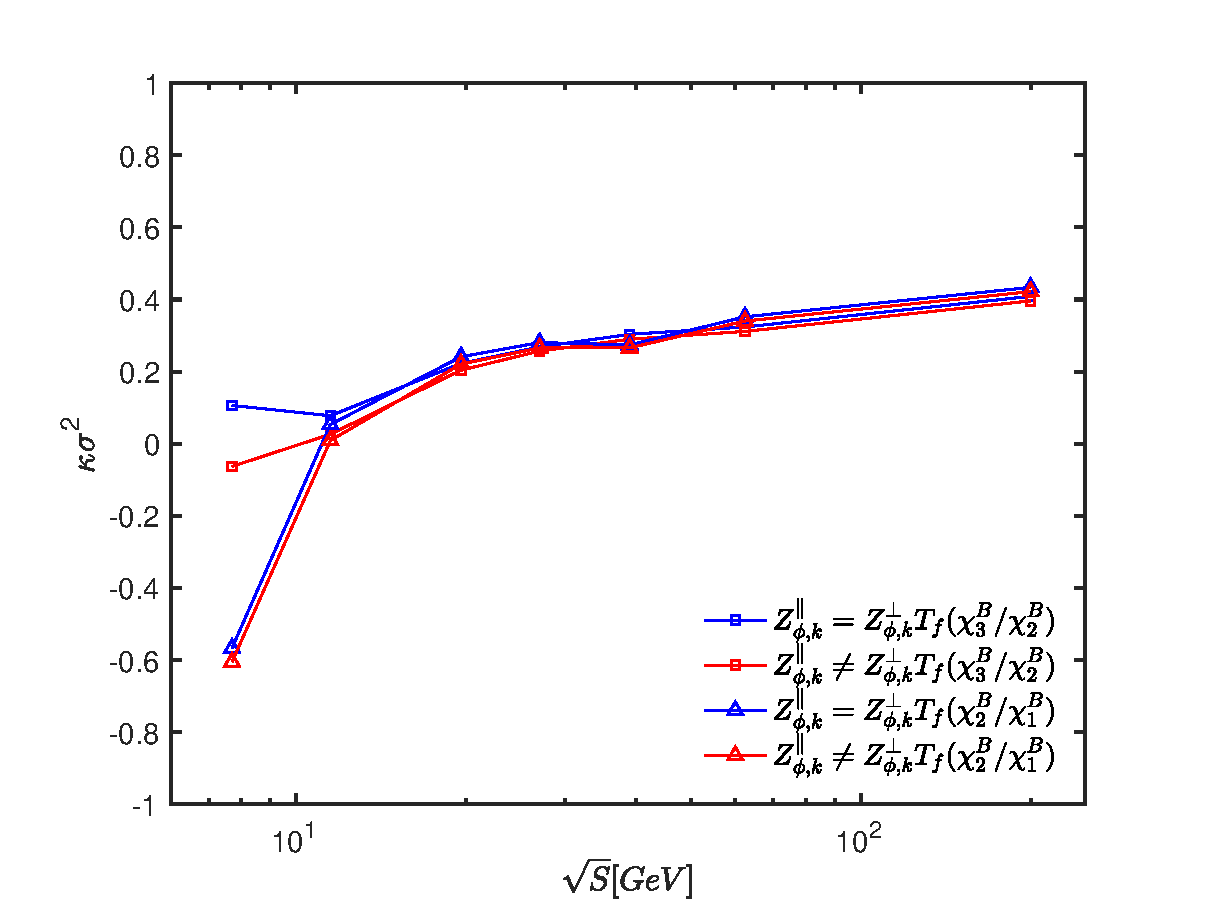
\includegraphics[width=0.46\textwidth]{freeze.eps}
\caption{blue color stands for the results with $Z^{\bot}_{\phi,k}=Z^{\|}_{\phi,k}$ and the red color stands for the $Z^{\bot}
_{\phi,k}\neq Z^{\|}_{\phi,k} $.}
\label{fig:freeze}
\end{figure}


%%%%%%%%%%%%%%%%%%%%%%%%%%%%%%%%%%%%
\section{summery and outlook}
In this work, we investigated the baryon number fluctuations and some thermodynamic quantities with in the functional 
renormalization group. We made a comparison of the results between the approximation of the mesonic wave function 
renormalizations and without the approximation. The calculation are accomplished under the fix point and physical point expansion of 
the effective potential. The result of the comparison is obvious, the approximation of the mesonic wave function renormalizations 
$Z^{\|}_{\phi}=Z^{\bot}_{\phi}$ cause few difference in the numerical computation, thus this approximation is good enough to use in 
the future work. And the different expansion methods of the effective potential do lead to some difference results of the meson mass.
%%%%%%%%%%%%%%%%%%%%%%%%%%%%%%%%%%%%
\acknowledgments
Thanks


%%%%%%%%%%%%%%%%%%%%%%%%%%%%%%%%%%%%

\appendix
\section{the regulator functions and the threshold functions}\label{a}
Three-d flat regulators have been used in this work. The regulator functions of the meson field and quark field can be 
written as
\begin{align}
\begin{split}
R^{\phi}_{k}(q_0,\vec{q})&=Z^{\bot}_{\phi,k}\vec{q}^2r_B(\vec{q}^2/k^2) ,\\
R^{q}_{k}(q_0,\vec{q})&=Z_{q,k}i\vec{\gamma}\cdot\vec{q}r_F(\vec{q}^2/k^2)
\end{split}
\end{align} 
in which
\begin{align}
\begin{split}
r_B(x)&=\left( \frac{1}{x}-1 \right)\Theta(1-x) ,\\
r_F(x)&=\left( \frac{1}{\sqrt{x}}-1 \right)\Theta(1-x)
\end{split}
\end{align} 
Then we give a definition to the meson and quark propagator
\begin{align}
\begin{split}
G_\phi(q,\bar{m}^{2}_{\phi,k})&=\frac{1}{z_\phi\tilde{q}^{2}_{0}+1+\bar{m}^{2}_{\phi,k}} ,\\
G_q(q,\bar{m}^{2}_{q,k})&=\frac{1}{z^{2}_{q}(\tilde{q}_0+i\tilde{\mu})^2+1+\bar{m}^{2}_{q,k}}
\end{split}
\end{align} 
in the equation above we have $\tilde{q}_0=q_0/k$, $\tilde{\mu}=\mu/k$ and for the fermions we have
$q_0=(2n_q+1)\pi T (n_q\in \mathbb{Z})$ for the bosons we have $q_0=2n_q\pi T$. Here $z=Z^\|/Z^\bot$ is the ratio of the 
two components of the wave function renormalizations. In this work we choose $z_q=1$ which means $Z^{\|}_{q}=
Z^{\bot}_{q}$ and $z_\phi\neq 1$ which means $Z^{\|}_{\phi}\neq Z^{\bot}_{\phi}$. To obtain the threshold functions, we 
define
\begin{align}
\begin{split}
\mathcal{F}_{(1)}(\bar{m}^{2}_{q,k},z_q;T,\mu)&=\frac{T}{k}\sum_{n_q}G_q(q,\bar{m}^{2}_{q,k}),\\
\mathcal{B}_{(1)}(\bar{m}^{2}_{\phi,k},z_\phi;T)&=-\frac{T}{k}\sum_{n_q}G_\phi(q,\bar{m}^{2}_{\phi,k})
\end{split}
\end{align} 
By summing the propagator up over the Matsubara frequencies, we can get the form of the definitions above
\begin{align}
\begin{split}
\mathcal{F}_{(1)}(\bar{m}^{2}_{q,k},z_q;T,\mu)=&\frac{1}{2z_q\sqrt{1+\bar{m}^{2}_{q,k}}}\times(1-n_F(\bar{m}^{2}_{q,k},z_q
;T,\mu)\\&-n_F(\bar{m}^{2}_{q,k},z_q;T,-\mu))
\end{split}
\end{align} 
and
\begin{align}
\begin{split}
\mathcal{B}_{(1)}(\bar{m}^{2}_{\phi,k},z_\phi;T)=&\frac{1}{z_\phi^{1/2}\sqrt{1+\bar{m}^{2}_{\phi,k}}}
(\frac{1}{2}-n_B(\bar{m}^{2}_{\phi,k},z_\phi;T)
\end{split}
\end{align} 
in the equations above the form of the distribution functions are
\begin{align}
\begin{split}
n_B(\bar{m}^{2}_{\phi,k},z_\phi;T)=\frac{1}{\mathbf{exp}\lbrace \frac{1}{T}\frac{k}{z_\phi^{1/2}}(1+\bar{m}^{2}_{\phi,k})^{1/2} 
\rbrace-1}
\end{split}
\end{align} 
and
\begin{align}
\begin{split}
n_F(\bar{m}^{2}_{q,k},z_\phi;T)=\frac{1}{\mathbf{exp}\lbrace \frac{1}{T}\frac{k}{z_q}(1+\bar{m}^{2}_{q,k})^{1/2}-\mu 
\rbrace+1}
\end{split}
\end{align} 
In the effective potential's flow equation, there are bosonic and fermionic threshold functions. The anomalous dimension 
of the mesonic field has change into the transverse component of it. The form of the threshold functions are
\begin{align}
\begin{split}
l_0^{(B,d)}(\bar{m}^{2}_{\phi,k},\eta^\bot_{\phi,k};T)=\frac{2}{d-1}\left( 1- \frac{\eta^{\bot}_{\phi,k}}{d+1}\right) 
\mathcal{B}_{(1)}(\bar{m}^{2}_{\phi,k},z_\phi;T)
\end{split}
\end{align} 
and
\begin{align}
\begin{split}
l_0^{(F,d)}&(\bar{m}^{2}_{q,k},\eta_{q,k};T,\mu)\\&=\frac{2}{d-1}\left( 1-\frac{\eta_{q,k}}{d} \right)\mathcal{F}_{(1)}
(\bar{m}^{2}_{q,k},z_q=1;T,\mu)
\end{split}
\end{align} 
Then, we define
\begin{align}
\begin{split}
\mathcal{F}_{(n)}(\bar{m}^{2}_{q,k},z_q;T,\mu)=\frac{T}{k}\sum_{(n_q)}(G_q(q,\bar{m}^{2}_{q,k}))^n
\end{split}
\end{align} 
and through the equation below we can deduce the expression of any value of $n$
\begin{align}
\begin{split}
\mathcal{F}_{(n+1)}(\bar{m}^{2}_{q,k},z_q;T,\mu)=-\frac{1}{n}\frac{\partial}{\partial\bar{m}^{2}_{q,k}}\mathcal{F}_{(n)}
(\bar{m}^{2}_{q,k},z_q;T,\mu)
\end{split}
\end{align} 
The definition of the threshold function $\mathcal{BB}_{(1,1)}$ is
\begin{align}
\begin{split}
\mathcal{BB}_{(1,1)}&(\bar{m}^{2}_{\phi_a,k},\bar{m}^{2}_{\phi_b,k},z_\phi;T)\\
&=-\frac{T}{k}\sum_{n_q}G_\phi(q,\bar{m}^{2}_{\phi_a,k})G_\phi(q,\bar{m}^{2}_{\phi_b,k})
\end{split}
\end{align} 
then we can obtain the $\mathcal{BB}_{(2,2)}$ in a same way
\begin{align}
\begin{split}
\mathcal{BB}_{(2,2)}&(\bar{m}^{2}_{\phi_a,k},\bar{m}^{2}_{\phi_b,k},z_\phi;T)\\
&=\frac{\partial^2}{\partial\bar{m}^{2}_{\phi_a,k}\partial\bar{m}^{2}_{\phi_b,k}}\mathcal{BB}_{(1,1)}(\bar{m}^{2}_{\phi_a,k}
\bar{m}^{2}_{\phi_b,k},z_\phi;T)
\end{split}
\end{align} 
The expression of the $\mathcal{BB}_{(1,1)}$ is 
\begin{widetext}
\begin{align}
\begin{split}
\mathcal{BB}_{(1,1)}(\bar{m}^{2}_{\phi_a,k},\bar{m}^{2}_{\phi_b,k},z_\phi;T)&=-\frac{1}{z^{1/2}_{\phi}}\left\{ \left( 
\frac{1}{2}+n_B(\bar{m}^{2}_{\phi_a,k},z_\phi;T) \right)\frac{1}{(1+\bar{m}^{2}_{\phi_a,k})^{1/2}} \right. \\
&\left.\times \frac{1}{\bar{m}^{2}_{\phi_a,k}-\bar{m}^{2}_{\phi_b,k}}+\left( \frac{1}{2}+n_B(\bar{m}^{2}_{\phi_b,k},z_\phi;T) 
\right)\right. \\
&\left.\times \frac{1}{(1+\bar{m}^{2}_{\phi_b,k})^{1/2}}\frac{1}{\bar{m}^{2}_{\phi_b,k}-\bar{m}^{2}_{\phi_a,k}}\right\}
\end{split}
\end{align} 
\end{widetext}
then we can get the expression of the threshold functions of any $n$.
At the same time, in our calculation there are also some other kind of threshold functions.
\begin{align}
\begin{split}
{\mathcal{BB}\tilde{q}_0^2}_{(1,1)}&(\bar{m}^{2}_{\phi_a,k},\bar{m}^{2}_{\phi_b,k},z_\phi;T)\\
&=-\frac{T}{k}\sum_{n_q}G_\phi(q,\bar{m}^{2}_{\phi_a,k})G_\phi(q,\bar{m}^{2}_{\phi_b,k})\tilde{q}_0^2
\end{split}
\end{align}
 The form of the threshold functions 
$\mathcal{F}\tilde{q}_0^2$,  $\mathcal{F}\tilde{q}_0^4$ and $\mathcal{BB}\tilde{q}_0^2$ is like



\begin{align}
\begin{split}
&{\mathcal{BB}\tilde{q}_0^2}_{(1,1)}(\bar{m}^{2}_{\phi_a,k},\bar{m}^{2}_{\phi_b,k},z_\phi;T)=\\
&-Z_\phi^{1/2}\left\{ \left( 
\frac{1}{2}+n_B(\bar{m}^{2}_{\phi_a,k},z_\phi;T) \right)\frac{(1+\bar{m}^{2}_{\phi_a,k})^{-1/2}}{\bar{m}^{2}_{\phi_b,k}-
\bar{m}^{2}_{\phi_a,k}}\right.\\
&\left.+\left( \frac{1}{2}+n_B(\bar{m}^{2}_{\phi_b,k},z_\phi;T) \right)\frac{(1+\bar{m}^{2}_{\phi_a,k})^{-1/2}}
{\bar{m}^{2}_{\phi_a,k}-\bar{m}^{2}_{\phi_b,k}}\right\}
\end{split}
\end{align} 



By using the method above we can get the threshold functions that contain the summation of fermion and boson 
propagators $\mathcal{FB}$ in the quark anomalous dimension.
\begin{widetext}
\begin{align}
\begin{split}
\mathcal{FB}&_{(1,1)}(\bar{m}^{2}_{q,k},\bar{m}^{2}_{\phi,k},z_q,z_\phi;T,\mu,p_0)\\
&=\frac{T}{k}\sum_{n_q}G_\phi(p-q,\bar{m}^{2}_{\phi,k})G_q(q,\bar{m}^{2}_{q,k})\\
&=\frac{1}{2}\frac{k^2}{z_\phi z^{2}_{q}} \left\{ -n_B(\bar{m}^{2}_{\phi,k},z_\phi;T)
\frac{z^{1/2}_{\phi}}{(1+\bar{m}^{2}_{\phi,k})^{1/2}}\frac{1}{\left( ip_0-\mu+\frac{k}{z^{1/2}_{\phi}}(1+\bar{m}^{2}_{\phi,k})
^{1/2} \right)-(1+\bar{m}^{2}_{q,k})(\frac{k}{z_q})^{2}}\right. \\
&\left.-(n_B(\bar{m}^{2}_{\phi,k},z_\phi;T)+1)\frac{z^{1/2}_{\phi}}{(1+\bar{m}^{2}_{\phi,k})^{1/2}}\frac{1}{\left( ip_0-\mu+
\frac{k}{z^{1/2}_{\phi}(1+\bar{m}^{2}_{\phi,k})} \right)^2-(1+\bar{m}^{2}_{q,k})(\frac{k}{z_q})^{2}}\right. \\
&\left.+n_F(\bar{m}^{2}_{q,k},z_q;T,-\mu)\frac{z_q}{(1+\bar{m}^{2}_{q,k})^{1/2}}\frac{1}{\left( ip_0-\mu-\frac{k}{z_q}(1+
\bar{m}^{2}_{q,k})^{1/2} \right)^2-(1+\bar{m}^{2}_{\phi,k})\frac{k^2}{z_\phi}}\right. \\
&\left.+(n_F(\bar{m}^{2}_{q,k},z_q;T,\mu)-1)\frac{z_q}{(1+\bar{m}^{2}_{q,k})^{1/2}}\frac{1}{\left( ip_0-\mu+\frac{k}{z_q}
(1+\bar{m}^{2}_{q,k})^{1/2} \right)^2-(1+\bar{m}^{2}_{\phi,k})\frac{k^2}{z_\phi}}\right\}
\end{split}
\end{align} 
\end{widetext}

%%%%%%%%%%%%%%%%%%%%%%%%%%%%%%%%%%%%%%%%%%%%%


\section{mesonic anomalous dimensions}\label{b}
In order to obtain the flow equation of the effective potential, the mesonic anomalous dimensions are needed. Because 
we have divided the wave function renormalizations into the transverse and longitudinal components of it, so the 
anomalous dimensions should be divided either.
The analytical form of the mesonic anomalous dimensions can be written like
\begin{align}
\begin{split}
\eta_{\phi,k}^{\|}&=\eta_{\phi,k}^{\|}(0,0)\\
&=\frac{1}{6\pi^2}\left\{ 
 \frac{4}{k^2z_\phi^4}\bar{\kappa}_k(\bar{V}''_k(\bar{\kappa}_k))^2\left[ 
 2\mathcal{BB}_{(2,2)}(\bar{m}^{2}_{\pi,k},\bar{m}^{2}_{\sigma,k};T)\right.\right.\\
&\left.\left.-4{\mathcal{BB}\tilde{q}^{2}_{0}}_{(2,3)}(\bar{m}^{2}_{\pi,k},\bar{m}^{2}_{\sigma,k};T)-4{\mathcal{BB}
\tilde{q}^{2}_{0}}_{(3,2)}(\bar{m}^{2}_{\pi,k},\bar{m}^{2}_{\sigma,k};T)\right]\right.\\
&\left.\times(1-\frac{1}{5}\eta^{\bot}_{\phi,k})+\frac{N_c\bar{h}^{2}_{k}}{z_\phi}\mathcal{F}_{(3)}(\bar{m}^{2}_{q,k};T,\mu)(4-\eta_{q,k})
\right\}   
\end{split}
\end{align} 
and the other component
\begin{align}
\begin{split}
\eta_{\phi,k}^{\bot}&=\eta_{\phi,k}^{\bot}(0,0)\\
&=\frac{1}{6\pi^2}\left\{ 
\frac{4}{k^2z_\phi^4}\bar{\kappa}_k(\bar{V}''_k(\bar{\kappa}_k))^2 \mathcal{BB}_{(2,2)}(\bar{m}^{2}_{\pi,k},\bar{m}^{2}_{\sigma,k};T)
\right.\\&\left.+N_c\bar{h}^{2}_{k}\left[\mathcal{F}_{(2)}(\bar{m}^{2}_{q,k};T,\mu)(2\eta_{q,k}-3)\right.\right.\\
&\left.\left.-4(\eta_{q,k}-2)\mathcal{F}_{(3)}(\bar{m}^2_{q,k};T,\mu)\right]
\right\}   
\end{split}
\end{align} 


%%%%%%%%%%%%%%%%%%%%%%%%%%%%%%%%%%%%%%%%%%%%

\section{Flow equations of the fermion}\label{c}
The flow of the quark wave function renormalization are given by
\begin{align}
\begin{split}
\eta_{q,k}(p_0,\vec{p})=&\frac{1}{Z_{q,k}(p_0,\vec{p})}\frac{1}{4N_cN_f}\\
&Re\left[\frac{\partial^2}{\partial|p|^2}Tr\left( i\vec{\gamma}\cdot \vec{p}\left( -\frac{\delta^2\partial_t\Gamma_k}
{\delta\bar{q}(-p)\delta q(p)} \right) \right)\bigg|_{\rho=\kappa}\right]
\end{split}
\end{align} 
and the flow of the Yukawa coupling can be written as
\begin{align}
\begin{split}
\partial_th_k(p_0,\vec{p})=&\frac{\sqrt{2N_f}}{\sigma}\frac{1}{4N_cN_f}\\
&\times Re\left[ Tr\left( -\frac{\delta^2\partial_t\Gamma_k}{\delta\bar{q}(-p)\delta q(p)} \right)\bigg|_{\rho=\kappa} \right]
\end{split}
\end{align} 






Now we can obtain the form of the quark anomalous dimension
\begin{align}
\begin{split}
\eta_{q,k}=&\frac{1}{24\pi^2N_f}(4-\eta_{\phi,k})\bar{h}^{2}_{k}\\
&\times\{ (N^{2}_{f}-1)\mathcal{FB}_{(1,2)}(\bar{m}^{2}_{q,k},\bar{m}^{2}_{\pi,k};T,\mu,p_{0,ex})\\
&+\mathcal{FB}_{(1,2)}(\bar{m}^{2}_{q,k},\bar{m}^{2}_{\sigma,k};T,\mu,p_{0,ex}) \}
\end{split}
\end{align} 


%%%%%%%%%%%%%%%%%%%%%%%%%%%%%%%%%%%%%%%%%%%%


































\end{document}